\documentclass[11pt]{standalone}
\usepackage{amssymb}
\usepackage{amsmath}
\usepackage[no-math]{fontspec}
\usepackage{unicode-math}
\usepackage{libertinus}
\usepackage{pgf,xcolor}
\usepackage{tikz}
\usetikzlibrary{arrows.meta, backgrounds, calc}
\usepackage{pgfplots}
\pgfplotsset{compat=newest}

% ── Color palette (all seven defined in every file) ──────────────────────────
\definecolor{my_darkgray}{HTML}{484949}
\definecolor{my_lightgray}{HTML}{F3F4F4}
\definecolor{my_darkblue}{HTML}{005A94}
\definecolor{my_lightblue}{HTML}{CCDEE9}
\definecolor{my_yellow}{HTML}{FFEC7F}
\definecolor{my_red}{HTML}{E60000}
\definecolor{my_orange}{HTML}{E87846}

\begin{document}
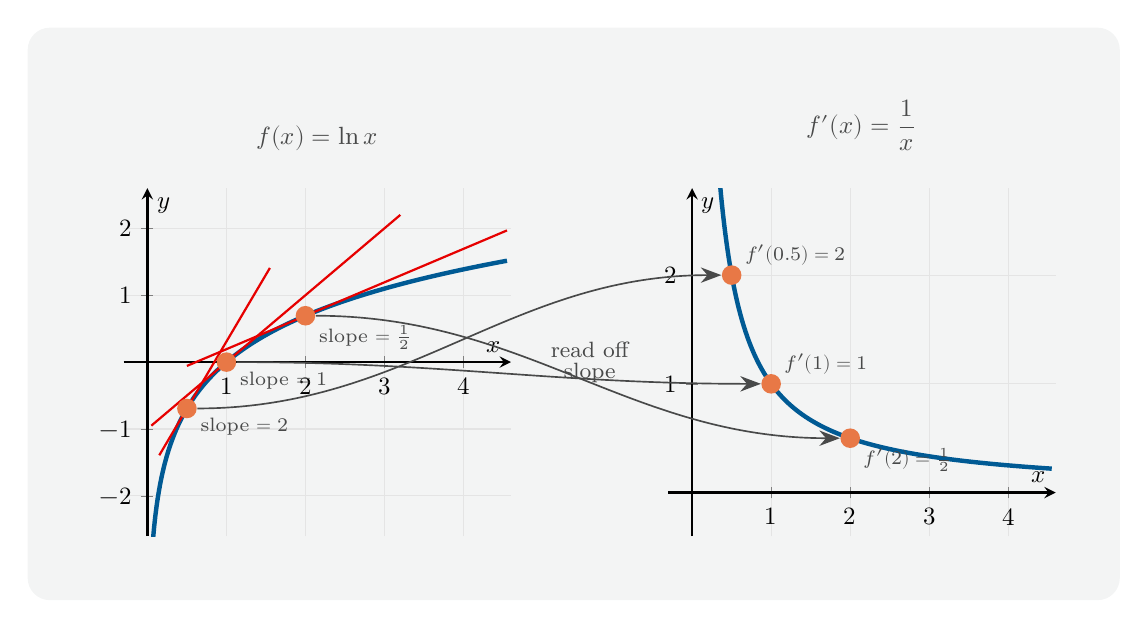
\begin{tikzpicture}[
    show background rectangle,
    background rectangle/.style={fill=my_lightgray, rounded corners=8pt},
    inner frame sep=0.8cm
]

% ── Left panel: f(x) = ln(x) with tangent lines at x = 0.5, 1, 2 ────────────
%
% axis equal omitted: y range [-2.5, 2.5] against x range [0, 4.5] would
% produce an unreadably wide panel at equal scale.
%
\begin{axis}[
    name             = ax_left,
    width            = 6.5cm,
    height           = 6.0cm,
    axis lines       = center,
    xlabel           = {$x$},
    ylabel           = {$y$},
    grid             = both,
    grid style       = {color=my_darkgray!15},
    xmin = -0.3,  xmax = 4.6,
    ymin = -2.6,  ymax = 2.6,
    axis line style  = {thick},
    title            = {$f(x) = \ln x$},
    title style      = {font=\small\bfseries, color=my_darkgray, yshift=4pt},
    tick label style = {font=\small},
    label style      = {font=\small},
    xtick            = {1,2,3,4},
    ytick            = {-2,-1,0,1,2},
]

  % Primary curve: ln(x), domain starts just above 0 to avoid the singularity
  \addplot[color=my_darkblue, samples=300, ultra thick,
           domain=0.04:4.55]{ln(x)};

  % Tangent at x=0.5: slope = 1/0.5 = 2, passes through (0.5, ln 0.5)
  %   y = ln(0.5) + 2*(x - 0.5)  =  2x - 1.693
  %   Domain clipped so the line stays within the visible y-range.
  \addplot[color=my_red, thick, domain=0.15:1.55]{2*x - 1.693};

  % Tangent at x=1: slope = 1, passes through (1, 0)
  %   y = x - 1
  \addplot[color=my_red, thick, domain=0.05:3.2]{x - 1};

  % Tangent at x=2: slope = 0.5, passes through (2, ln 2)
  %   y = ln(2) + 0.5*(x - 2)  =  0.5x - 0.307
  \addplot[color=my_red, thick, domain=0.5:4.55]{0.5*x - 0.307};

  % ── Sample point markers (also named export nodes) ───────────────────────
  \node[circle, fill=my_orange, inner sep=2.5pt] (L1)
      at (axis cs:0.5, {ln(0.5)}) {};
  \node[circle, fill=my_orange, inner sep=2.5pt] (L2)
      at (axis cs:1, 0) {};
  \node[circle, fill=my_orange, inner sep=2.5pt] (L3)
      at (axis cs:2, {ln(2)}) {};

  % ── Slope annotations ────────────────────────────────────────────────────
  \node[font=\scriptsize, color=my_darkgray, anchor=north west]
      at (axis cs:0.55, {ln(0.5)})
      {slope $= 2$};
  \node[font=\scriptsize, color=my_darkgray, anchor=north west]
      at (axis cs:1.05, 0)
      {slope $= 1$};
  \node[font=\scriptsize, color=my_darkgray, anchor=north west]
      at (axis cs:2.05, {ln(2)})
      {slope $= \tfrac{1}{2}$};

\end{axis}

% ── Right panel: f'(x) = 1/x ─────────────────────────────────────────────────
\begin{axis}[
    name             = ax_right,
    at               = {(ax_left.east)},
    anchor           = west,
    xshift           = 2.0cm,
    width            = 6.5cm,
    height           = 6.0cm,
    axis lines       = center,
    xlabel           = {$x$},
    ylabel           = {$y$},
    grid             = both,
    grid style       = {color=my_darkgray!15},
    xmin = -0.3,  xmax = 4.6,
    ymin = -0.4,  ymax = 2.8,
    axis line style  = {thick},
    restrict y to domain=-0.5:3.5,   % safety net near the singularity
    title            = {$f'(x) = \dfrac{1}{x}$},
    title style      = {font=\small\bfseries, color=my_darkgray, yshift=4pt},
    tick label style = {font=\small},
    label style      = {font=\small},
    xtick            = {1,2,3,4},
    ytick            = {0,1,2},
]

  % Derivative curve: 1/x, positive branch only (domain of ln x)
  % Start at 0.35 so that 1/0.35 ≈ 2.86 stays within ymax = 2.8.
  \addplot[color=my_darkblue, samples=300, ultra thick,
           domain=0.35:4.55]{1/x};

  % ── Derivative value markers ──────────────────────────────────────────────
  \node[circle, fill=my_orange, inner sep=2.5pt] (R1)
      at (axis cs:0.5, 2) {};
  \node[circle, fill=my_orange, inner sep=2.5pt] (R2)
      at (axis cs:1, 1) {};
  \node[circle, fill=my_orange, inner sep=2.5pt] (R3)
      at (axis cs:2, 0.5) {};

  % ── Derivative value annotations ─────────────────────────────────────────
  \node[font=\scriptsize, color=my_darkgray, anchor=south west]
      at (axis cs:0.55, 2)
      {$f'(0.5) = 2$};
  \node[font=\scriptsize, color=my_darkgray, anchor=south west]
      at (axis cs:1.05, 1)
      {$f'(1) = 1$};
  \node[font=\scriptsize, color=my_darkgray, anchor=north west]
      at (axis cs:2.05, 0.5)
      {$f'(2) = \tfrac{1}{2}$};

\end{axis}

% ── Arrows from sample points on left to derivative values on right ───────────
% The two panels have different y-ranges, so the arrows curve: the steep slope
% at x = 0.5 (left, near the bottom) maps to the large value 1/0.5 = 2 (right,
% near the top); the gentle slope at x = 2 maps to the small value 1/2 (right,
% near the bottom). The changing direction of the arrows visually encodes the
% fact that the derivative 1/x is a decreasing function.
\draw[-{Stealth[scale=1.3]}, color=my_darkgray, semithick]
    (L1) to[out=0, in=180] (R1);
\draw[-{Stealth[scale=1.3]}, color=my_darkgray, semithick]
    (L2) to[out=0, in=180] (R2);
\draw[-{Stealth[scale=1.3]}, color=my_darkgray, semithick]
    (L3) to[out=0, in=180] (R3);

% ── Label in the arrow gap ────────────────────────────────────────────────────
\node[font=\footnotesize, color=my_darkgray, align=center]
    at ($(ax_left.east)!0.5!(ax_right.west)$)
    {read off\\[-2pt]slope};

\end{tikzpicture}
\end{document}
